%%%%%%%%%%%%%%%%%%%%%%%%%%%%%%%%%%%%%%%%%%%%%%%%%%%%%%%%%%%%%%%%%%%%%%%
%%%%  Load the document class and packages                         %%%%
%%%%%%%%%%%%%%%%%%%%%%%%%%%%%%%%%%%%%%%%%%%%%%%%%%%%%%%%%%%%%%%%%%%%%%%
\documentclass[a4paper]{report}
\usepackage{epsfig}            % to insert PostScript figures
\graphicspath{ 
	{./figures/} 
}

%Change figure names
\renewcommand{\figurename}{Fig}

\usepackage[bf,footnotesize]{caption} % make captions small and label bold

\addtocounter{chapter}{1} %Because starting at zero is silly
\makeatletter
\renewcommand{\thesection}{\@arabic\c@section}
\renewcommand{\thefigure}{\@arabic\c@figure}
\makeatother

\usepackage{titlesec} %change spacing before and after sections
%format: \titlespacing*{<command>}{<left>}{<before-sep>}{<after-sep>}
\titlespacing*{\section}{0pt}{11mm plus 1ex minus .2ex}{6mm plus .2ex}
\titlespacing*{\subsection}{0pt}{9mm plus 1ex minus .2ex}{4mm plus .2ex}

\usepackage[a4paper,margin=3.7cm,tmargin=2.5cm,bmargin=2.5cm]{geometry} 
\usepackage{textcomp}          % To make nice degree symbols and others\usepackage[bf,footnotesize]{caption} % make captions small and label bold
\usepackage{wrapfig}
%to produce the clickable references along the left in Acroread. This
%package must be included last. 
\usepackage[ps2pdf,bookmarks=TRUE]{hyperref} 
\hypersetup{
    colorlinks=true,
    linkcolor=cyan,
    filecolor=magenta,      
    urlcolor=cyan,
}
\usepackage{wrapfig}

%%%%%%%%%%%%%%%%%%%%%%%%%%%%%%%%%%%%%%%%%%%%%%%%%%%%%%%%%%%%%%%%%%%%%%%
%%%%  Hypertext references for Acrobat                             %%%%
%%%%%%%%%%%%%%%%%%%%%%%%%%%%%%%%%%%%%%%%%%%%%%%%%%%%%%%%%%%%%%%%%%%%%%%
\hypersetup{
	pdfauthor = {SWC},
	pdftitle = {Optics Exercises},
	pdfkeywords = {optics, lenses, refraction, reflection, dispersion,
		telescope, microscope},
	pdfcreator = {LaTeX with hyperref},
	pdfproducer = {dvips + ps2pdf}
}

%%%%%%%%%%%%%%%%%%%%%%%%%%%%%%%%%%%%%%%%%%%%%%%%%%%%%%%%%%%%%%%%%%%%%%%
%%%%  Main text                                                    %%%%
%%%%%%%%%%%%%%%%%%%%%%%%%%%%%%%%%%%%%%%%%%%%%%%%%%%%%%%%%%%%%%%%%%%%%%%
\begin{document}
	
	%set the number of sectioning levels 
	\setcounter{secnumdepth}{2}
	
	\begin{center}
		\textbf{\Large{Image Formation}}
	\end{center}
	
	%%%%%%%%%%%%%%%%%%%%%%%%%%%%%%%%%%%%%%%%%%%%%%%%%%%%%%%%%%%%%%%%%%%%%%%
%	\section{Introduction}
	%%%%%%%%%%%%%%%%%%%%%%%%%%%%%%%%%%%%%%%%%%%%%%%%%%%%%%%%%%%%%%%%%%%%%%%
	\vspace{0.8cm}
	\noindent The goal of this series of exercises is to gain an intuition of what lenses do and how they can be combined on a simple optical setup. 
	
% 	\begin{itemize}
% 	    \item Bullet points are things to do
% 	    \item Hints are at the end of the document. Click on `Go to hint' and `Go back' to navigate. Don't just read the hint right away, but be sure to read it before moving on.
% 	    \item Help with the assembly of optics parts can be found in `Assembly Instructions'.
% 	\end{itemize}

%     current ToDos \\
%   - add phone pixel size question?
%   - add wavefront sensor question
% 	- add justification of thin lens approximation, paraxial rays etc.? \\
% 	- this goes into abberrations, where to treat them? just leave it to the lecture? \\
% 	- make assembly pics and put in 'General Instruction' \\
% 	- figure out laser pointer alignment problem \\
% 	- finish hint for telescope \\
% 	- finish hints for challenge questions \\
% 	- add question with sensor size? use basler acA1440-220um vs. acA2040-120um
	

    %%%%%%%%%%%%%%%%%%%%%%%%%%%%%%%%%%%%%%%%%%%%%%%%%%%%%%%%%%%%%%%%%%%%%%%
	\section{Image formation -- quick recap}
	%%%%%%%%%%%%%%%%%%%%%%%%%%%%%%%%%%%%%%%%%%%%%%%%%%%%%%%%%%%%%%%%%%%%%%%
	\hypertarget{hintBack-recap}{}
    
     Figure~\ref{fig:raytracerules} illustrates the three rules of ray-tracing through an ideal convex (positive) lens. 
     By definition, convex lenses focus parallel rays to a spot at a distance of 1 focal length from the lens. 
     The is illustrated by rules A and B, which are equivalent (B is the reverse of A). 
     Rule C shows the special case where the angle of the ray leaving the lens is the same as the angle of the ray entering the lens. 
     

	\begin{figure}[h]
		\center
		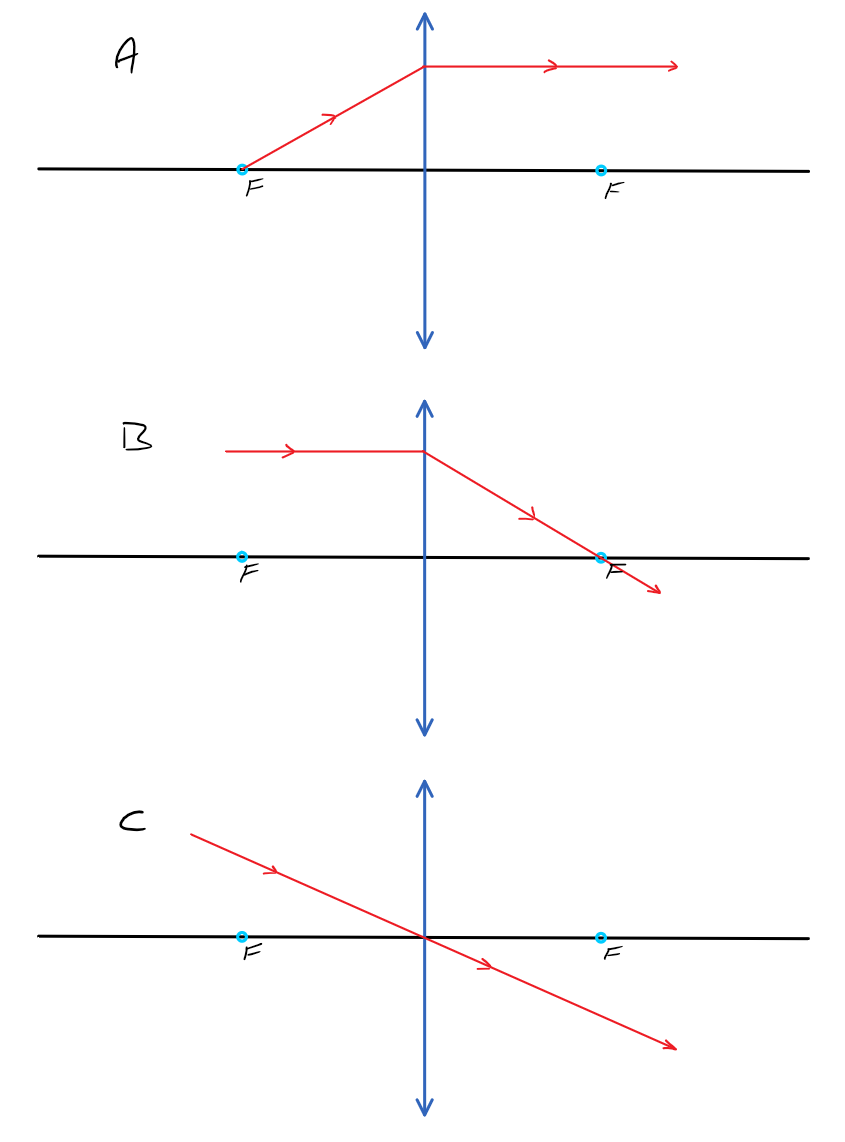
\includegraphics[width=0.8\textwidth]{figures/ray_trace_rules.png}
		\captionsetup{width=0.95\textwidth}
		\caption{The three rules of ray-tracing through a thin convex lens.
		\textbf{A}. Rays (red) originating from the front focal point exit the lens parallel to the optical axis (black line).
		\textbf{B}. Rays entering the lens parallel to the optical axis will pass through the rear focal point.
		\textbf{C}. Rays traveling through the centre of the lens are not deviated: leaving the lens at the same angle at which they entered it. 
		}
		\label{fig:raytracerules}
	\end{figure}
	
	\clearpage 
	
	\textbf{An image is formed when light rays leaving one point of an object converge again at another point in space}.
	This is illustrated in Fig.~\ref{fig:imageforming}, where the penguins on the left are imaged through an idealised thin lens. 
	Two of the privileged rays from Fig.~\ref{fig:raytracerules} are shown for each penguin object:
	\begin{itemize}
	\item The color-coded rays correspond to the undeviated case shown in Fig.~\ref{fig:raytracerules}C. 
	\item The exiting black ray corresponds to Fig.~\ref{fig:raytracerules}B: it enters the lens parallel to the optical axis and gets refracted to the focal point.
	\end{itemize}
	Note how all penguins share the second, parallel, ray -- it thus becomes easily apparent how the image-forming condition varies according to the angle of the centre ray. 
	
	\begin{figure}[h]
		\center
		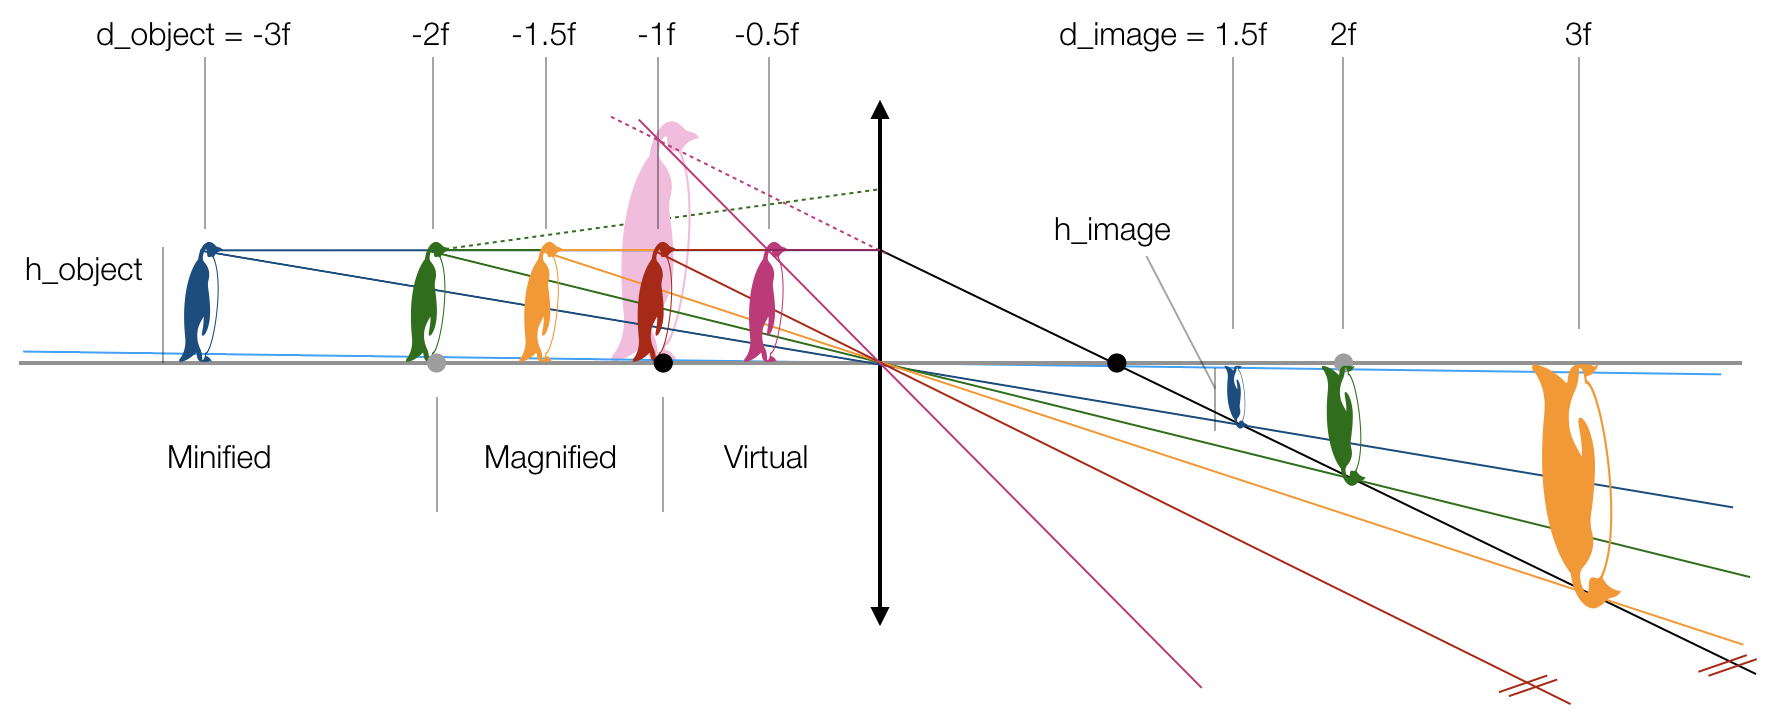
\includegraphics[width=1\textwidth]{figures/penguin_lens.png}
		\captionsetup{width=0.95\textwidth}
		\caption{Image formation using an idealised thin lens with focal length $f$. Object and image distance are shown in function of $f$. 
		The light blue ray close to the optical axis illustrates how, for $d_o$ close to infinity, the image will be formed ever closer to the focal point (this ray comes from a very distant penguin's beak).
		}
		\label{fig:imageforming}
	\end{figure}
	
	\noindent
	Where the image forms is given by the thin lens equation: 
	\begin{equation}
	\frac{1}{f} = \frac{1}{d_i} - \frac{1}{d_o}
	\label{eq:thinlens}
	\end{equation}
	
	Sign conventions follow Cartesian coordinates (objects placed to the left of the lens are at negative distances). For positive (convex) lenses, $f>0$. For negative (concave) lenses, $f<0$.

	\begin{itemize}
	    \item Convince yourself that the thin lens equation matches the ray tracing
	    \item We assert that \emph{all rays} (not just the `privileged rays' used for tracing) leaving a point on the penguin's head and passing through the lens will meet again in the image plane. Check this by tracing a random ray, such as the green dotted ray leaving the green penguin in Fig.~\ref{fig:imageforming}. 
	\end{itemize}
	

    \clearpage

	%%%%%%%%%%%%%%%%%%%%%%%%%%%%%%%%%%%%%%%%%%%%%%%%%%%%%%%%%%%%%%%%%%%%%%%
	\section{Please meet the lens}
	%%%%%%%%%%%%%%%%%%%%%%%%%%%%%%%%%%%%%%%%%%%%%%%%%%%%%%%%%%%%%%%%%%%%%%%
	
	%----------------------------------------------------------------------
    \subsection{Determine the focal length of a convex lens}
    %----------------------------------------------------------------------
	\hypertarget{hintBack-focal_length}{}
	Your optics kit contains a number of small plastic boxes, each containing a lens whose focal length may or may not match what is printed on its box. 
	How can you estimate the focal length of a lens and thereby determine whether it matches what is stated on the box? 
	(There is an easy / approximate way of doing this using just the one lens.)

	
	
	%----------------------------------------------------------------------
    \subsection{Forming an image with a lens}
    %----------------------------------------------------------------------
	\hypertarget{hintBack-image}{}
	As you are reading this, the lenses in your eyes are forming images of the text onto the retina. 
	In the room, we don't have a closed space like the eye to shield the detector from stray light, making it hard to see images of the room formed by a lens onto a piece of paper (stray light reduces \emph{contrast}). 
	So we will use a bright LED as an object -- this will allow us to see the image of the LED emitter formed on a piece of paper.
	
	\subsubsection{Setting up the LED}
	Your first task is to set up the LED on the optical rail:
	\begin{itemize}
    \item Attach a post holder to a rail carriage (Fig. 1) and place this on the rail.
    \item Attach a 50 mm post to the white LED glued to a cage plate and place this in the post holder.
    \item Power the LED using the ThorLabs LED driver and LED power cable.
	\end{itemize}

	\subsubsection{Forming an image of the LED emitter}
	Choose any lens and mount it in a lens holder using the lens tool. 
	Mount the lens on the rail with a second carriage, post, and post holder. 
	You can form an image of the LED emitter on a white card or you can use the plastic post-mountable screen. 
	
    \begin{itemize}
	    \item What expectations do you have about image formation based on Fig. \ref{fig:imageforming}? Verify that these are true by forming images of the LED emitter on the card for different values of $d_o$. (The LED emitter looks like a small square with dots in a grid -- if all you see is a blur, you are not looking at an image)
	    \item Under what circumstances will you \emph{not} form an image of the emitter? Draw the ray diagram and try it on the rail.
	    \item The magnification of the object in the image plane is given by  $m = h_i / h_o = d_i / d_o$. $m=1$ indicates unitary magnification. Negative indicate an inverted image. 
	    Optional: Use similar triangles in Fig. \ref{fig:imageforming} to derive a formula for magnification with the known quantities $f$ and $d_o$.
		\item Use the setup to measure the size of the LED emitter.
	\end{itemize}

    \clearpage

	\subsubsection{Forming an image of a distant source}
    Use a lens of about $f=60~mm$ to form an image of the room lights on a piece of paper.
    The image will be formed at very close to $1f$.
    Repeat with a lens of about $f=200~mm$. 
    What two things do you notice about the images produced by these lenses? 
    Fig.~\ref{fig:outside} models the situation you saw. 
    Can you explain your observations using these ray diagrams?
    
    
    \begin{figure}[h]
    \center
    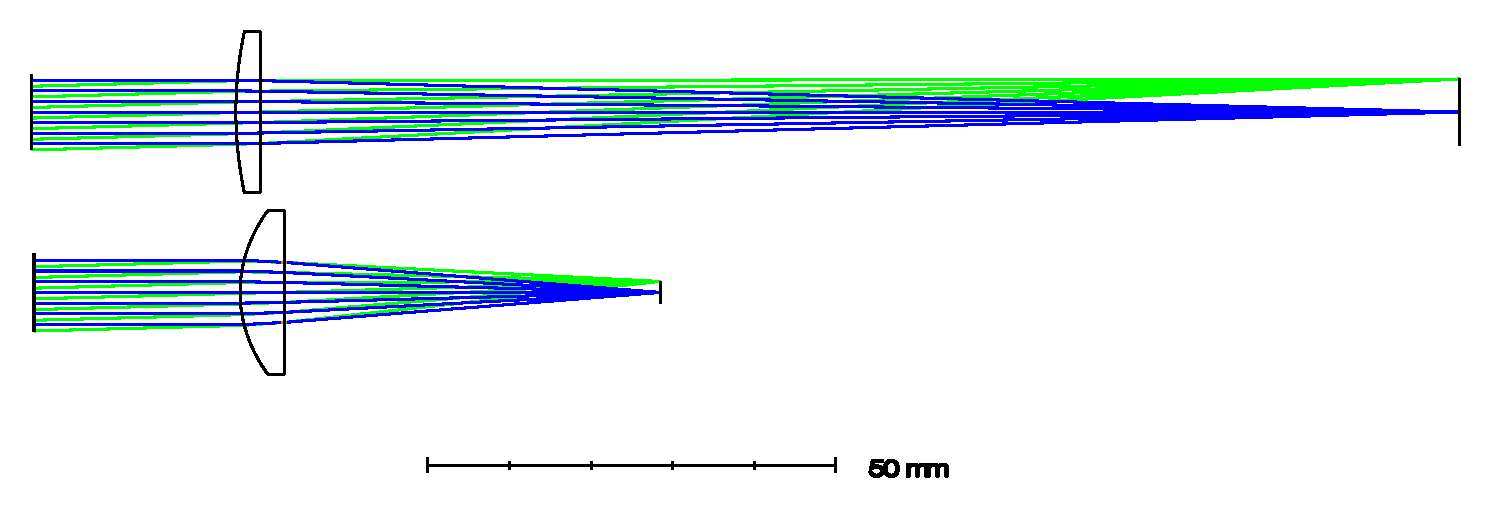
\includegraphics[width=6in]{figures/lens_f_comparison.eps}
    \caption{Images formed at $1f$ from light originating at infinity. 
    The top is a $f=150~mm$ lens and the bottom a $f=50~mm$ lens.
    Light from different regions of the object arrive in parallel rays that come in at different angles (green and blue). 
    Each set of parallel rays come into focus at a point, satisfying the image-forming condition. }
    \label{fig:outside}
    \end{figure}

	
	%----------------------------------------------------------------------
    \subsection{Virtual images}
    %----------------------------------------------------------------------
    \hypertarget{hintBack-virtual}{}
    The images you have formed above are \emph{real images}, meaning that they are created by rays which are \emph{converging}.
    In other words, a real image is a collection of focus points that is created by converging rays. 
    A \emph{virtual image}, on the other hand, is composed of a collection of points whose rays are \emph{diverging}.
    Unlike real images, virtual images can not be projected onto a screen and require an additional lens in order to achieve this. 
    
    Figure~\ref{fig:mirror} shows how a flat mirror forms a virtual image of an object apparently positioned behind the mirror. 
    The rays seem to diverge from points behind the mirror and the image is not magnified: the object appears to be as far behind the mirror as the object is in front of the mirror.
    The image of the bottle is only formed once rays are converged by a positive lens and focused on to a screen (e.g. as in the observer's eye).

    \begin{figure}[h]
    \center
    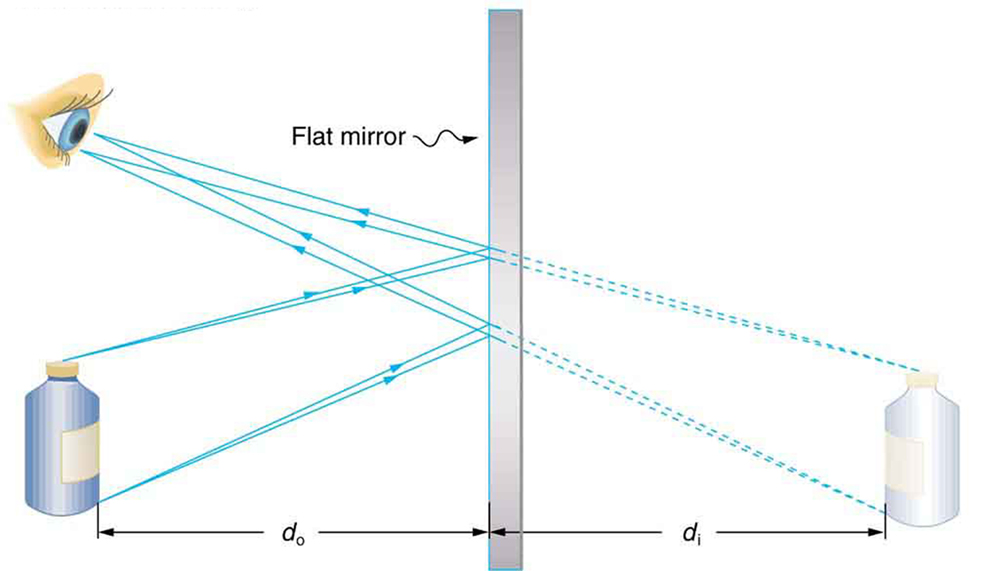
\includegraphics[width=4in]{figures/virtual_image_mirr.jpg}
    \caption{A virtual image of the bottle is created on the far side of the mirror. 
    This is described by the dotted lines which are `extended rays' that are used to form the virtual image. }
    \label{fig:mirror}
    \end{figure}
    
    \clearpage

    Light rays from a virtual image are angled such that they \emph{appear} to emanate from a point in the virtual image plane, but they never actually met in that point.
    This is seen starkly in Fig.~\ref{fig:negative_lens_tracing}, which is the ray diagram for a negative (concave) lens.

    \begin{figure}[h]
		\center
		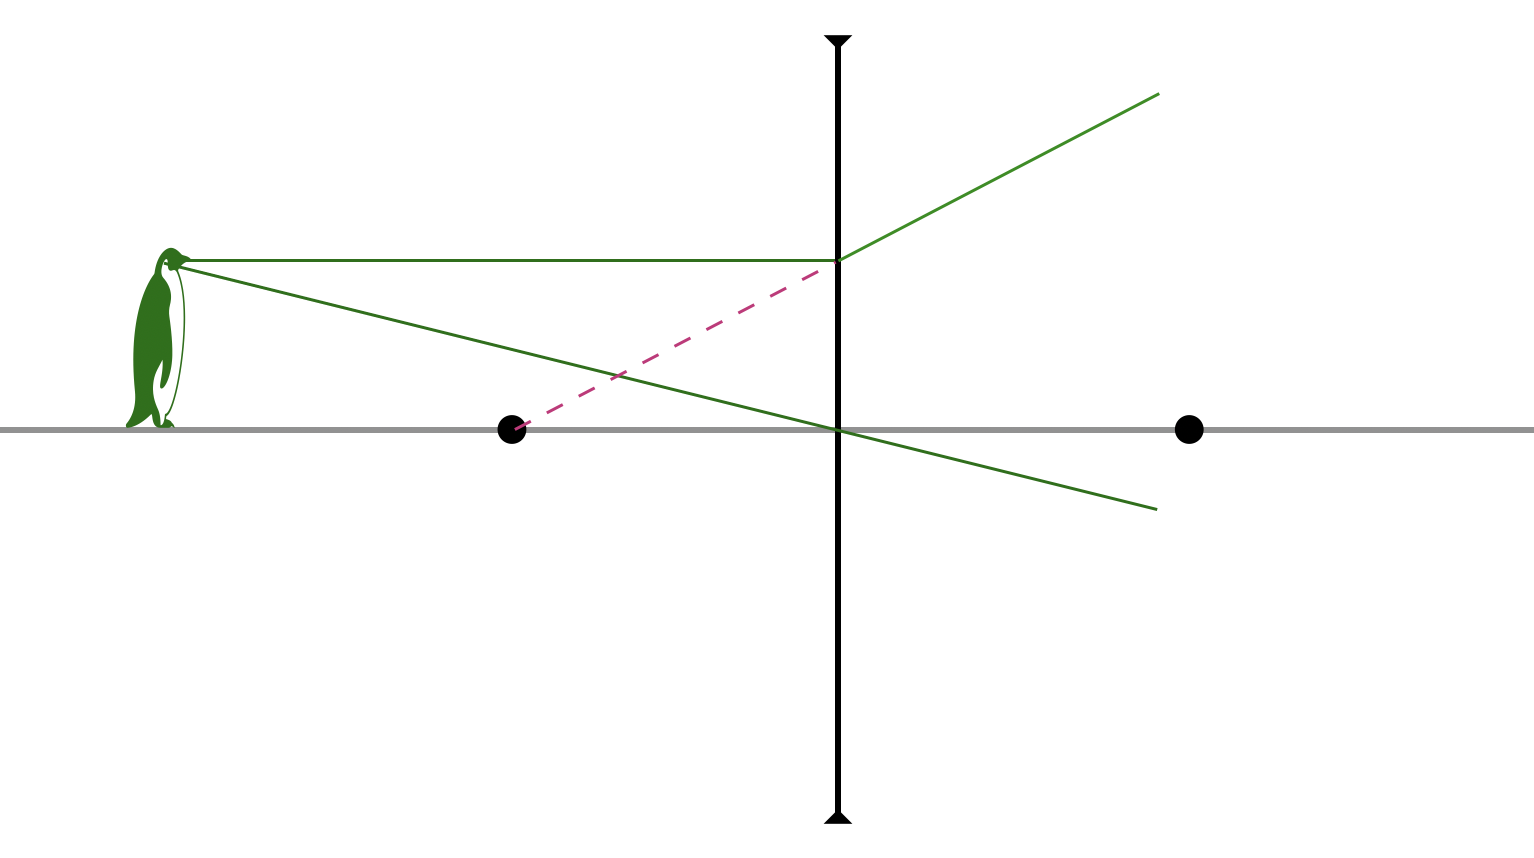
\includegraphics[width=0.5\textwidth]{figures/negative_lens_tracing.png}
		\captionsetup{width=0.6\textwidth}
		\caption{Ray tracing for a negative lens. The `identity' of the focal points is swapped compared to a positive lens -- the green ray parallel to the optical axis hits the lens and is drawn down to the focal point \emph{on the same (object) side}, as shown in dotted pink. This gives you the angle of the ray after the lens. \emph{Rays from the penguin's beak appears to emanate from the point where the dotted ray meets the ray going through the centre of the lens}.
		}
		\label{fig:negative_lens_tracing}
	\end{figure}

    \begin{itemize}
        \item Can you form a virtual image with a positive (convex) lens? If so, draw the ray diagram. 
        \item Check this with your own eyes (look through the lens at an object). Is this configuration ever used in daily life?
        \item Imagine (draw) what you see for $d_0$ close to $f$? See if you are right.
        \item Can you tell whether a lens is negative (diverges parallel light) or positive (converges parallel light) without using light, just by looking at the shape?
        \item What will you see if you look through a negative (concave) lens? Draw a ray diagram (don't forget your eye as the second lens). Check your expectations with the $f=-50mm$ lens from your kit.
        \item You might find an unlabeled negative lens - how could you determine its focal length?
    \end{itemize}

    \clearpage
	
	
	%%%%%%%%%%%%%%%%%%%%%%%%%%%%%%%%%%%%%%%%%%%%%%%%%%%%%%%%%%%%%%%%%%%%%%%
	\section{Multiple lenses}
	%%%%%%%%%%%%%%%%%%%%%%%%%%%%%%%%%%%%%%%%%%%%%%%%%%%%%%%%%%%%%%%%%%%%%%%
	
	You have seen that a lot can be done with a single lens: it can form images of different magnification and even create virtual images. 
	However, the real power of optical systems only becomes apparent when we chain together sequences of lenses. 
	In this scenario the image created by an upstream lens acts as the object to be imaged by a downstream lens.
	We will now examine two important scenarios that arise from pairs of lenses: the \emph{finite conjugate} configuration and the \emph{infinite conjugate} configuration. 
	\textbf{You will encounter these configurations again and again throughout the course}.
	
	%----------------------------------------------------------------------
	\subsection{Infinite conjugate configuration}
	%----------------------------------------------------------------------
	\hypertarget{hintBack-infinite}{}
	
	Let's begin with the `infinite conjugate', which is built using two lenses. 
	The term `conjugate` refers to the correspondence between the object and image planes. 
	The term `infinite` indicates that the lens forming the image does so with an object located at infinity.
	Thus, the object conjugated with the image is at infinity. 

	\begin{itemize}
		\item Draw a ray diagram of two lenses with $f_1=2 \cdot f_2$, $f_1$ apart, with an object at $-f_1$ of the first lens. Where does the image form? 
		\item Increase the distance between the lenses to $2\cdot f_1$ and redraw (or use another color on the same drawing), using the ray tracing rules. Where does the image form now? What happened to the magnification?
		\item What is the magnification of the image? Deduce the formula using similar triangles in your ray diagram.
		\item What could be the use of such a two-lens system in infinite conjugate configuration?
	\end{itemize}

    \noindent
	Let's verify your predictions on the rail with two lenses of your choice.  
	
	\begin{itemize}    
	    \item First, ensure the first lens is at $f_1$ from the LED (the object) before placing the second lens. You could use a ruler, but it can be hard to know where to measure from (where the optical centre of your lens is). What is a smarter way of doing it?
	    \item Place the second lens, and find where the image forms.
	    \item Verify the infinite space by moving the second lens and finding again with the screen where the image forms. Are your expectations met?
	\end{itemize}


	
	
	%----------------------------------------------------------------------
	\subsection{Beam expanders}
	%----------------------------------------------------------------------
	\hypertarget{hintBack-expand}{}
	
	Lasers are wonderful devices that produce light that is \emph{collimated}, or parallel. The idealised depiction is a beam of a certain width that stays parallel (in reality, they always expand / diverge to some degree). Before the invention of lasers in 1960, microscopy was much worse off.
	
    \begin{itemize}
        \item Can you collimate your LED? Draw the ray diagram.
		\item For reasons discussed later, the diameter of a laser beam in an optical system may need to be adjusted. Come up with a way to change the width of a collimated laser beam -- draw the ray diagram. What determines the size change? Deduce a formula from your diagram. 
	    \item Can you accomplish the task using a positive and a negative lens? 
	\end{itemize}

    \noindent
	To build the beam expander on the rail, we will i) align the laser diode to the rail using an iris, and ii) align the lenses with respect to the aligned beam. 


    \noindent
	Aligning the laser to the rail:
	\begin{itemize}
	    \item Check the `Assembly Instructions' to set up the rail, laser and iris.
	    \item Understand and implement the procedure depicted in Fig. \ref{fig:laser_alignment}. Iterate between the close and far position until the beam is straight.
	\end{itemize}


	\begin{figure}[h]
		\center
		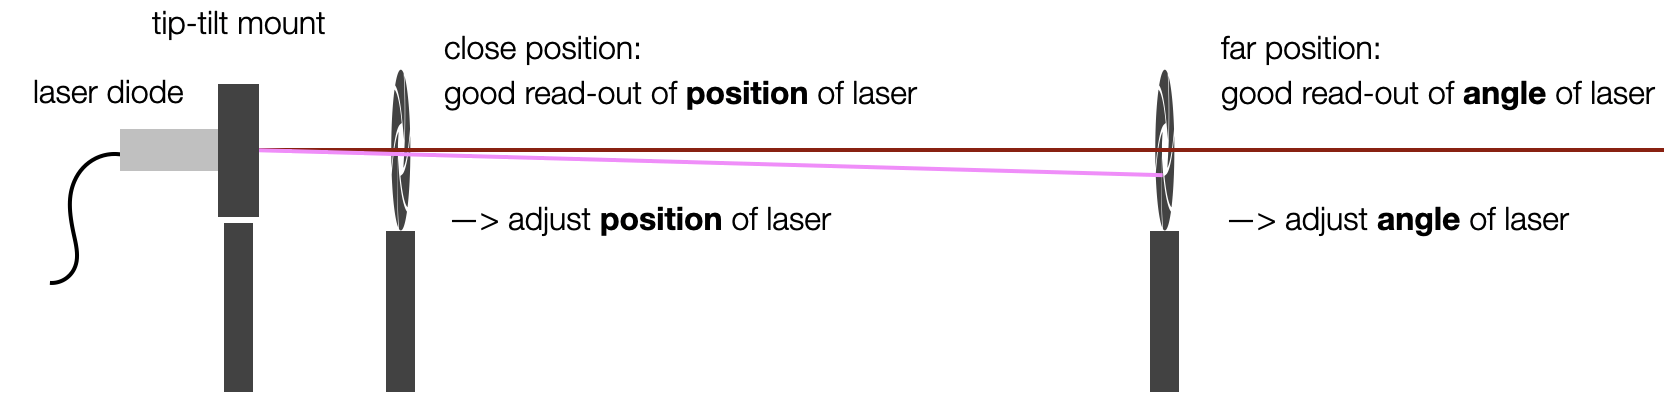
\includegraphics[width=0.9\textwidth]{figures/laser_alignment.png}
		\captionsetup{width=0.9\textwidth}
		\caption{Aligning the laser using a translating iris on the rail. When the iris is up against the laser, the angle of the beam changes little where it hits the iris -- but the height and lateral position matter a lot. Conversely, when the iris is far away, the angle of the beam matters most. Thus, the iris in close position allows you to find the correct position in space of the laser that intersects the imaginary line passing through the irises; the iris in far position allows you to find the correct angle of the beam.}
		\label{fig:laser_alignment}
	\end{figure}
	
	\noindent
	Placing of the beam expander:
	\begin{itemize}
	    \item \textbf{Coarse alignement:} First align by eye as best as you can -- all optical elements should be placed straight and centred at the same height. Use a ruler to ensure approximate distance between lenses is correct.
		\item \textbf{Fine alignment:} The lens is at the correct height if the beam still hits the iris centred after the lens is in place (assuming the laser is aligned!). You can also look at the back reflection from the lens, which should go straight back to the laser if all is straight (use lens paper to see the beam path).
		\item How can you ensure the two lenses are $f_1+f_2$ apart?
        \item Build a beam expander to yield the maximum magnification your optics kit allows.
		\item The beam expander you have built also goes by another common name.  What is it? 
		Think about what happens to beams that do not travel on-axis (Fig.~\ref{fig:telescope}). Once you've figured it out, remove the laser pointer, unfasten the rail and use your device.
	\end{itemize}


	
	\begin{figure}[h]
		\center
		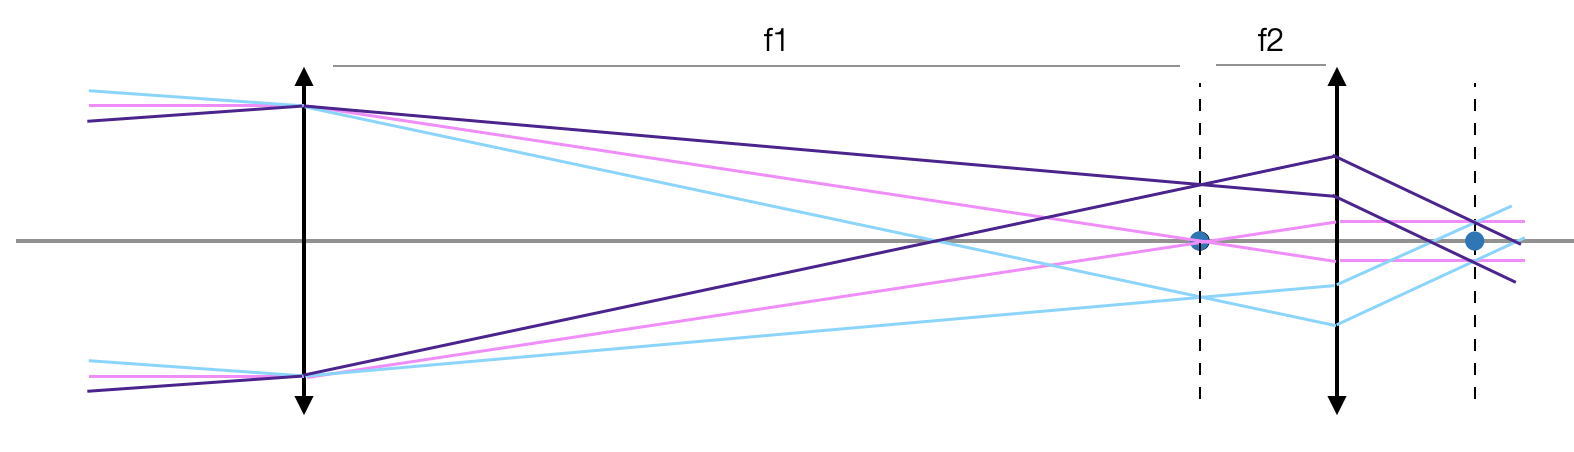
\includegraphics[width=0.9\textwidth]{figures/telescope.png}
		\captionsetup{width=0.9\textwidth}
		\caption{A Beam expander. In addition to the collimated beam arriving on-axis (pink), two off-axis beams are shown in different colors. Note how the angles of the beams leaving the second lens are amplified.}
		\label{fig:telescope}
	\end{figure}
	
	\clearpage
	%%%%%%%%%%%%%%%%%%%%%%%%%%%%%%%%%%%%%%%%%%%%%%%%%%%%%%%%%%%%%%%%%%%%%%%
	\section{Challenge questions}
	%%%%%%%%%%%%%%%%%%%%%%%%%%%%%%%%%%%%%%%%%%%%%%%%%%%%%%%%%%%%%%%%%%%%%%%
	
	%----------------------------------------------------------------------
    \subsection{Four lenses challenge}
    %----------------------------------------------------------------------
	Arrange 4 lenses, one of which must be a negative lens, so as to form a de-magnified, real, upright image. Reason through it, and remember that the image formed by the first lens is the object for the second, and so on. Pointers: 
	\begin{itemize}
    	\item For an object, use a glass slide with an arrow painted on the frosty label end. Collimate your LED first to get as much light from it as possible - a lot will be lost along the way. Illuminate the arrow from behind.
		\item Space will be a problem: the lenses will take up the whole rail and so you will need to place the target and screen outside of the rail.
		\item Do coarse alignment - look at your setup from the side / top and ensure all optical elements are centered with respect to each other
		\item There are multiple solutions to this problem.
	\end{itemize}
	There is no hint for this one...
	
	
	%----------------------------------------------------------------------
    \subsection{Buying a camera lens}
    %----------------------------------------------------------------------
    \hypertarget{hintBack-buying}{}
    The new raspberry pi high quality cameras are priced at 50\$, and you get excited about filming your setup from three perspectives. However, you need to choose a lens...
    
    \begin{itemize}
        \item Your friend mentions you should make sure to get a lens with a focus ring - what does the focus ring adjust? (both physically speaking and with respect to the thin lens equation)
        \item You find an unlabeled lens and wonder if it will be any good. Your friend has an idea: take a picture of her so she just fills the view, check how far away she stands, and deduce from that the focal length. Is she making any sense?
        \item You find a spare $f=50mm$ lens with fixed focus, but your friend asserts that you won't be able to focus on the mouse inside your 1m tall setup -- is she correct?
        \item You want to film your head-fixed mice up-close to track the pupil diameter. You can find three lenses online, with $f=6mm$, $f=16mm$ and $f=35mm$ -- which one do you choose? What if you want to film a 30cm wide arena from the ceiling of your 1m tall box?
    \end{itemize}

    
    
	%----------------------------------------------------------------------
    \subsection{A light-weight high NA lens}
    %----------------------------------------------------------------------
	\hypertarget{hintBack-fresnel}{}
	
	Large diameter high NA lenses can become quite bulky and sometimes very heavy. For example, look at the $60mm$ or $75mm$ 2 inch diameter lens in your kit; such lenses can be very impractical to use. Yet they are very useful to collimate light, as shown in Fig. \ref{fig:lighthouse_mirage}, where the light of a large revolving lamp is collimated for ships to see.
	
	\begin{itemize}
	    \item Explain how a lens could work that focuses light but has the dimensions of a credit card (flat and thin). As always, draw the ray diagrams and use concepts that were discussed.
	\end{itemize}


	

	%----------------------------------------------------------------------
    \subsection{A mirage for neuroscience}
    %----------------------------------------------------------------------
	\hypertarget{hintBack-mirage}{}
	
	On a hot day you may witness a strange phenomenon called a mirage: you can see a sort of reflection of distant objects on the ground, for example a car reflected on the road it is driving on as shown in Fig. \ref{fig:lighthouse_mirage}. 
	
	\begin{itemize}
	    \item Explain how a mirage works, with ray diagrams and concepts that were discussed. Why are mirages seen in the distance near the horizon?
	    \item This principle is used with great success in neuroscience to form images of cells deep in the brain -- do you know in which technique? How does it work?
	\end{itemize}

	
	
	\begin{figure}[h]
		\center
		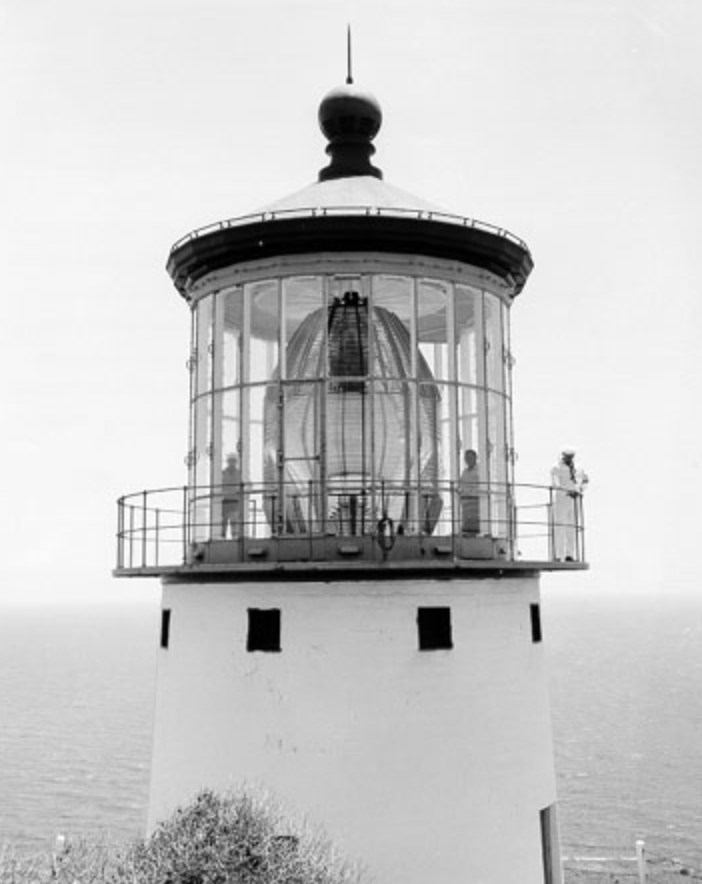
\includegraphics[width=0.2\textwidth]{figures/lighthouse.png}
		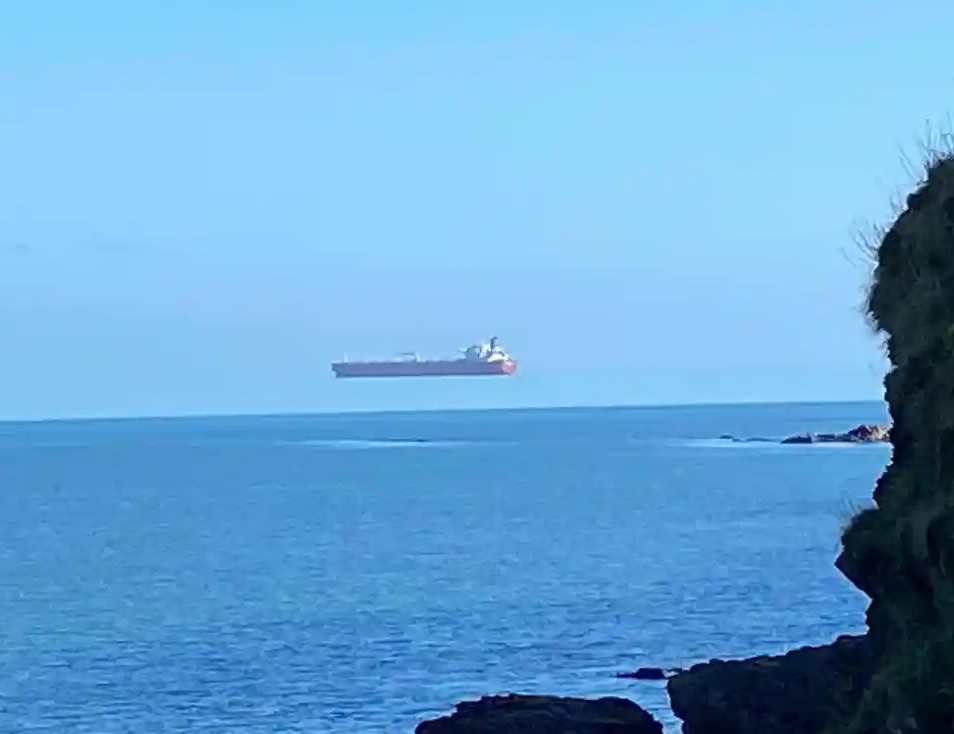
\includegraphics[width=0.327\textwidth]{figures/superior_mirage.png}
		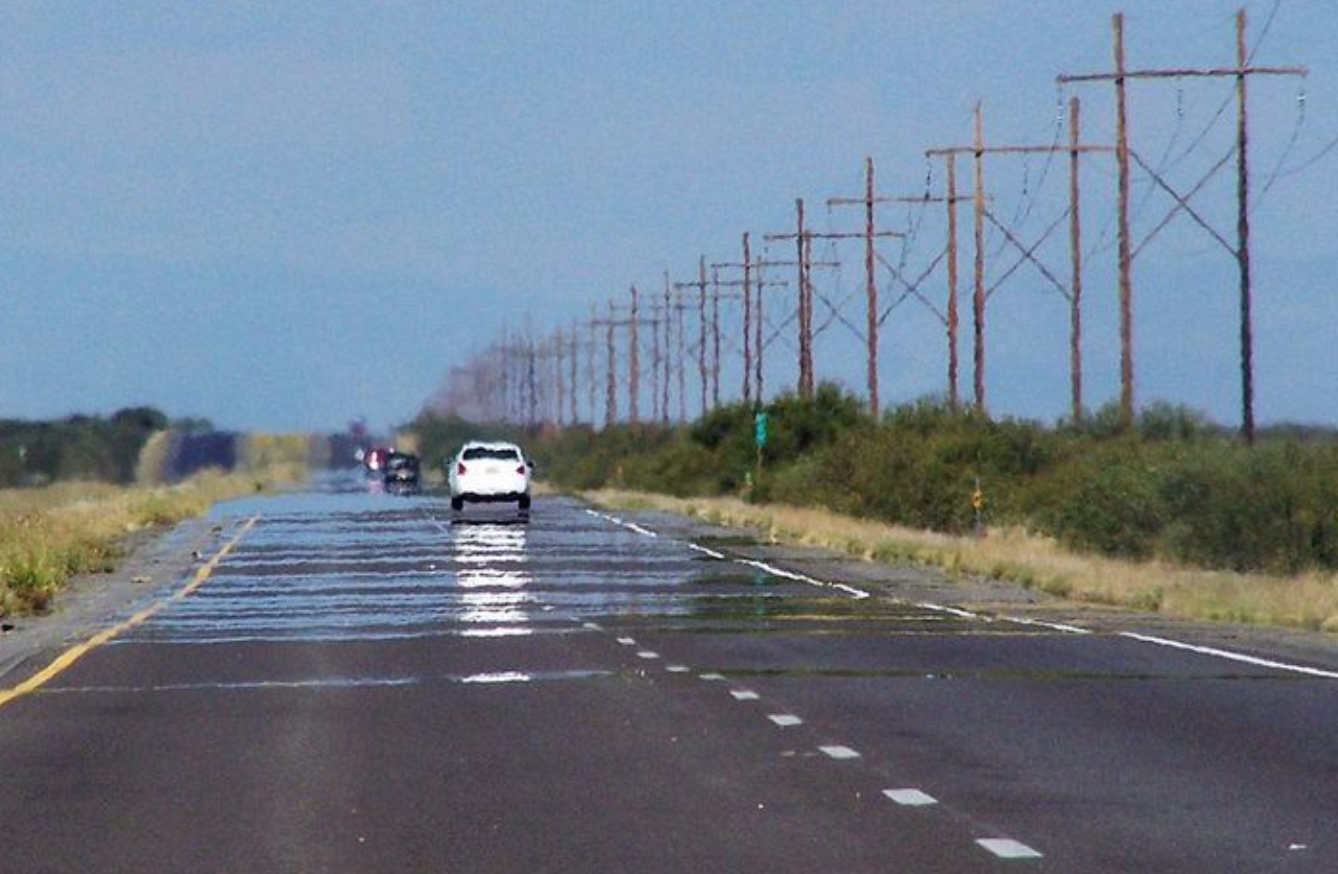
\includegraphics[width=0.385\textwidth]{figures/mirage.png}
		\captionsetup{width=0.93\textwidth}
		\caption{\emph{Left}: A lighthouse with a large high NA lens to collimate light from a lamp at its centre (source: wikipedia). 
		\emph{Middle}: A mirage at sea (photo credit: David Morris).
		\emph{Right}: A mirage on a street (photo credit: Joe Orman).}
		\label{fig:lighthouse_mirage}
	\end{figure}
	
	
	%----------------------------------------------------------------------
    \subsection{Rainbows}
    %----------------------------------------------------------------------
    Explain how rainbows form. What about double rainbows? Draw a sketch.
	
	
	\clearpage
	
	
	%%%%%%%%%%%%%%%%%%%%%%%%%%%%%%%%%%%%%%%%%%%%%%%%%%%%%%%%%%%%%%%%%%%%%%%
	\section{Image Formation: Answers, Hints, and Help}
	%%%%%%%%%%%%%%%%%%%%%%%%%%%%%%%%%%%%%%%%%%%%%%%%%%%%%%%%%%%%%%%%%%%%%%%
	
	%----------------------------------------------------------------------
    \subsection{Hint - Image formation recap}
    %----------------------------------------------------------------------
	\hypertarget{hintTo-recap}{}
	Using helper rays that obey the ray tracing rules we can trace the blue dotted ray shown below. By design of the lens, parallel rays will meet in the focal plane: the dotted ray going through the center of the lens thus defines where the ray we intend to trace must intersect the focal plane. By extension, all light emitted from the penguin's beak will be focused to the point in the imaging plane.
	\\
	
	Another view on tracing the blue ray: How light is bent by the lens is described by snell's law of refraction: $n_1 sin(\theta_1) = n_2 sin(\theta_2)$. For paraxial rays (travelling close to the optical axis and roughly parallel to it) encountering a thin lens (one that does not have a very curved surface), $sin(\theta)\cong\theta$, giving $n_1 \theta_1 = n_2 \theta_2$. In other words, the entering and exit angles of the beam are \emph{linearly} related. The pink ray can now be used to trace the blue dotted ray: for small angles, the light will be bent by a particular angle at that point on the lens, regardless of the angle of incidence. The pink and blue ray will travel at the same angle with respect to each other before and after the lens (note this is not quite true in the image, because the drawing is not within the paraxial/thin lens approximation, i.e. the ray is being bent by a large angle).
	
	\begin{figure}[h]
		\center
		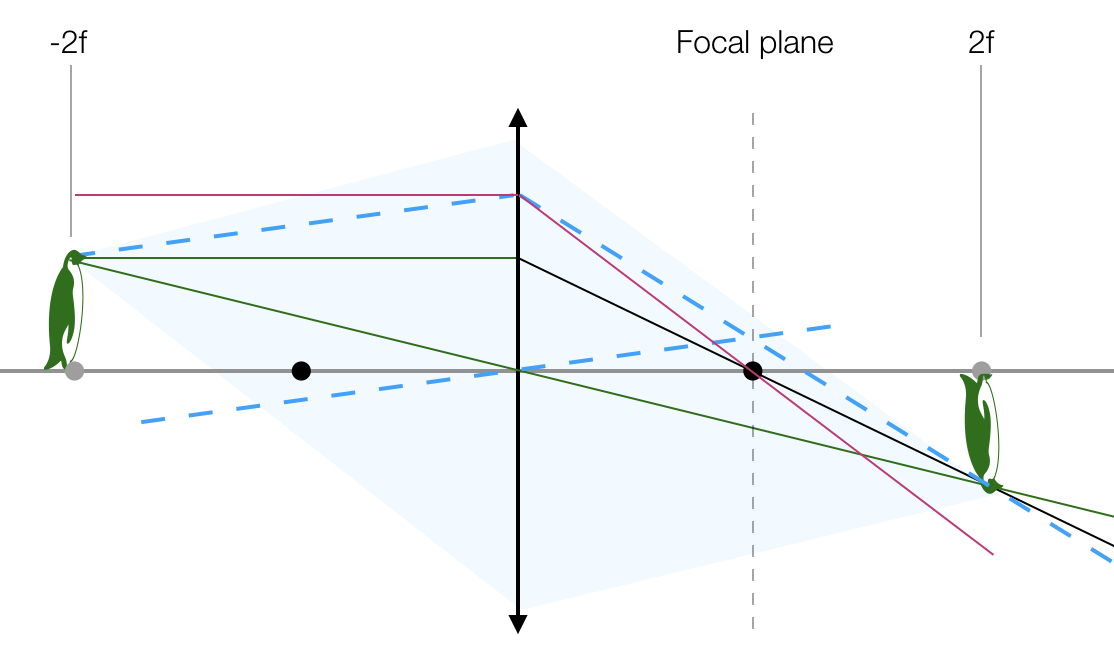
\includegraphics[width=0.75\textwidth]{hint_ray_tracing.png}
		\label{hint_ray_tracing}
	\end{figure}


    \clearpage
    
    
	%----------------------------------------------------------------------
    \subsection{Hint - Determining the focal length of a lens}
    %----------------------------------------------------------------------
	\hypertarget{hintTo-focal_length}{}
    Use the ray diagram shown in Fig. \ref{fig:imageforming} as starting point. If the object is quite far away compared to the focal length of the lens, where does the image form? In this case, rays arriving from a far away point at the lens are almost parallel to the optical axis -- they meet very close to the focal plane of the lens (see the blue and light blue rays in Fig. \ref{fig:imageforming})! Thus, we can use the sun as distant object, for which $d_i = f$. 
    
    Indoors, the ceiling lights will also do. Using the thin lens equation eq. \ref{eq:thinlens}, we can calculate the error in our measurement of $f$ if the object is at $d_o = 10f$ away instead of at near infinity: $s_i = 1.11f$, so we are 11\% off
    
    What is really happening when you use a magnifying glass on a sunny day to burn a hole in a piece of paper? You are forming a tiny image of the sun, concentrating all rays hitting the lens in a small area. 
    
    More generally, if you know the object distance $d_o$ and measure where the image forms $d_i$, you can deduce $f$ using the thin lens equation \ref{eq:thinlens}.


    \clearpage
    
    %----------------------------------------------------------------------
    \subsection{Hint - Image formation on the rail}
    %----------------------------------------------------------------------
	\hypertarget{hintTo-image}{}

    \subsubsection{A formula for magnification}
	Based on the similar triangles in Fig. \ref{fig:imageforming}, the magnification of a lens is calculated as follows:
	
	\begin{equation}
	M = \frac{h_i}{h_o} = \frac{d_i}{d_o} = \frac{f}{d_o+f}
	\label{eq:mag}
	\end{equation}
	
	A value of $M=1$ would mean unitary magnification (the image is the same size as the object), and negative numbers indicate an inverted image. For example, for $d_o=-2f$, this should match your observation on the rail that the magnification $m=-1$ (of course with the LED as object you can't tell if the image is inverted).
	\\
	\hyperlink{hintBack-image}{Go back}
	
	\subsubsection{Sizing up the emitter}
	There are many solutions to this. You could randomly place the LED and lens $d_o$ apart, and measure image size and distance $h_i$ and $d_i$, deduce the magnification factor and hence actual size of the emitter. However, ideally you should magnify the emitter so as to better be able to measure it on the screen -- so choosing $d_o=-1.5f$ would be a good start.


	
	\subsubsection{Forming no image}
	Recall the definition of an image-forming condition: \emph{light rays leaving one point of the object all meet again at some other defined point}. No image is formed when the LED is at $d_o=-f$, since rays leaving the lens are parallel and do not converge on the other side. Indeed, the thin lens equation tells us the image forms at infinity.


	\clearpage
	
	%----------------------------------------------------------------------
    \subsection{Hint - Virtual images}
    %----------------------------------------------------------------------
	\hypertarget{hintTo-virtual}{}
	
	\subsubsection{An observable virtual penguin}
	Rays coming from a point $d_o<f$ have angles that are too extreme (with respect to the optical axis) for the lens to bend sufficiently -- they exit the lens divergent. Imagine looking through the lens with the object at $d_o=-0.5f$, as illustrated in Fig. \ref{fig:imageforming} for the magenta penguin. While the rays don't actually emanate from a point, they certainly look like they do -- which is the same to your eyes! Your eyes will simply form an image of this virtual object (which is the virtual image formed by the first lens in this two lens system) \emph{as though it was really there}. 


	
	\subsubsection{A magnifying glass is just another lens}
	You are holding a magnifying glass -- which is simply any positive lens held $<f$ from the object. The virtual image, conveniently, is upright. As you can see from Fig. \ref{fig:imageforming}, if you push your magnifying glass against the object it looses its purpose and $M=1$. As you approach $d_o=f$, things become quite funky -- you can't see the object anymore, that is, you are seeing it with $M=inf$.


	
	\subsubsection{Positive and negative lenses}
	Positive lenses slow down light most near the optical axis where the lens is thickest -- negative lenses have the opposite net shape: there is more glass towards the rim than the centre (Fig. \ref{fig:lens_wave}). 
	
	\begin{figure}[h]
		\center
		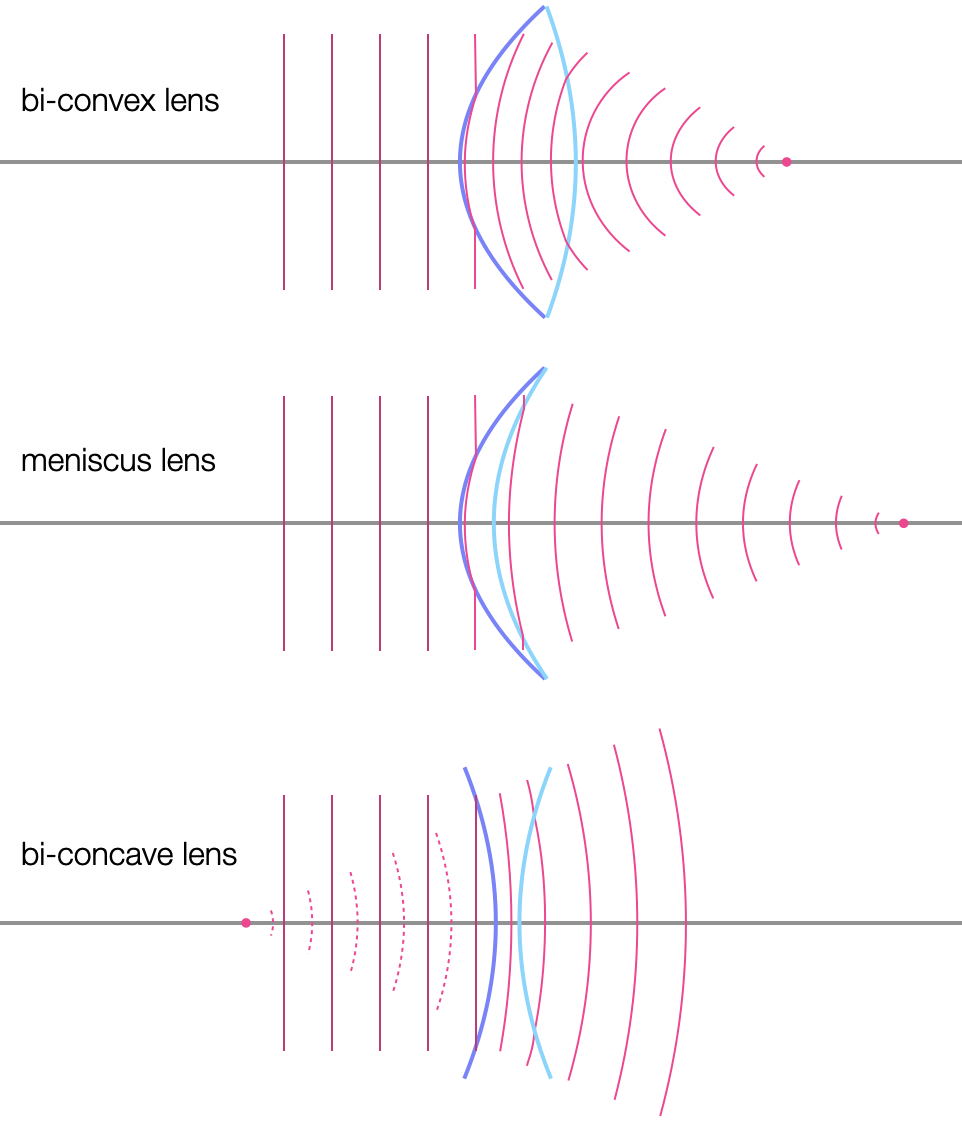
\includegraphics[width=0.55\textwidth]{figures/lens_wave_picture.png}
		\captionsetup{width=0.6\textwidth}
		\caption{Sketch of how collimated light is affected by two different lenses. Both are convex, because their center is wider than their edge. Planar wavefronts are therefore most slowed down in the center and converge to a point (if the lenses have the correct shape). Note how the wavelength is shorter inside the glass, because the speed of light is slower (does this mean it is a different color?).}
		\label{fig:lens_wave}
	\end{figure}

	
	\subsubsection{Looking through a negative lens, and how to find out its focal length}
	When you look through a negative lens, you see a small version of the world that is right-side-up -- no matter where the object is. In Fig. \ref{fig:neglens} the second lens would be your eyes ($d_o = 2\cdot f_{eye}$ was chosen for convenience).

	
	To determine the focal length of a negative lens, you need a second, positive lens (like your eyes): where the image forms will tell you about $d_i$ of the virtual image formed by the negative lens. 


    
	\begin{figure}[h]
		\center
		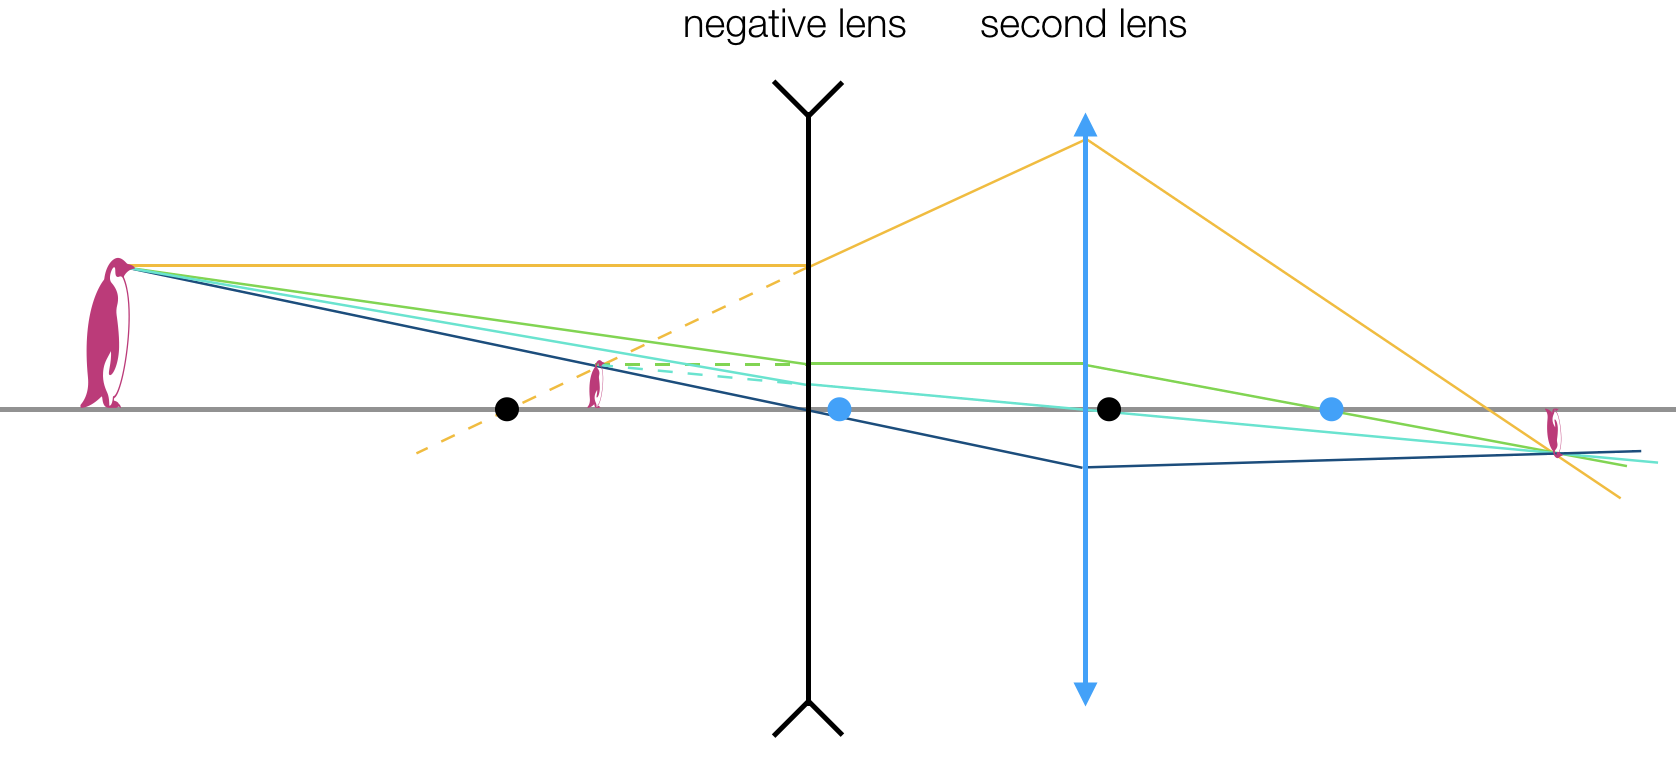
\includegraphics[width=0.9\textwidth]{figures/negative_lens.png}
		\captionsetup{width=0.9\textwidth}
		\caption{Ray diagram of someone looking through a negative lens. Dotted lines are never traversed by light emanating form the penguins beak. The yellow and dark blue rays are used to determined where the virtual image forms, which is the object for the second lens. The cyan and green rays are used to determined where the virtual penguin is imaged by the second lens.}
		\label{fig:neglens}
	\end{figure}
	
	
    \clearpage
    
    
    %----------------------------------------------------------------------
    \subsection{Hint - Infinite conjugate}
    %----------------------------------------------------------------------
	\hypertarget{hintTo-infinite}{}
	
	\subsubsection{Just another ray diagram}
	We use a helper ray (dotted ray in Fig. \ref{hint_infinite}) going parallel to the rays in infinite space and intersecting the middle of the second lens. The helper ray makes apparent that the image will form where this ray intersects the focal plane -- and is thus independent of the distance between the lenses. It solely depends on the angle of incident light, which is determined by $h_o$ and $f_1$.
	
	The magnification of the image is simply the ratio of the focal lengths (similar triangles again): 
	\begin{equation}
	M=-\frac{f_2}{f_1}
	\label{eq:magIC}
	\end{equation}
	
	\begin{figure}[h]
		\center
		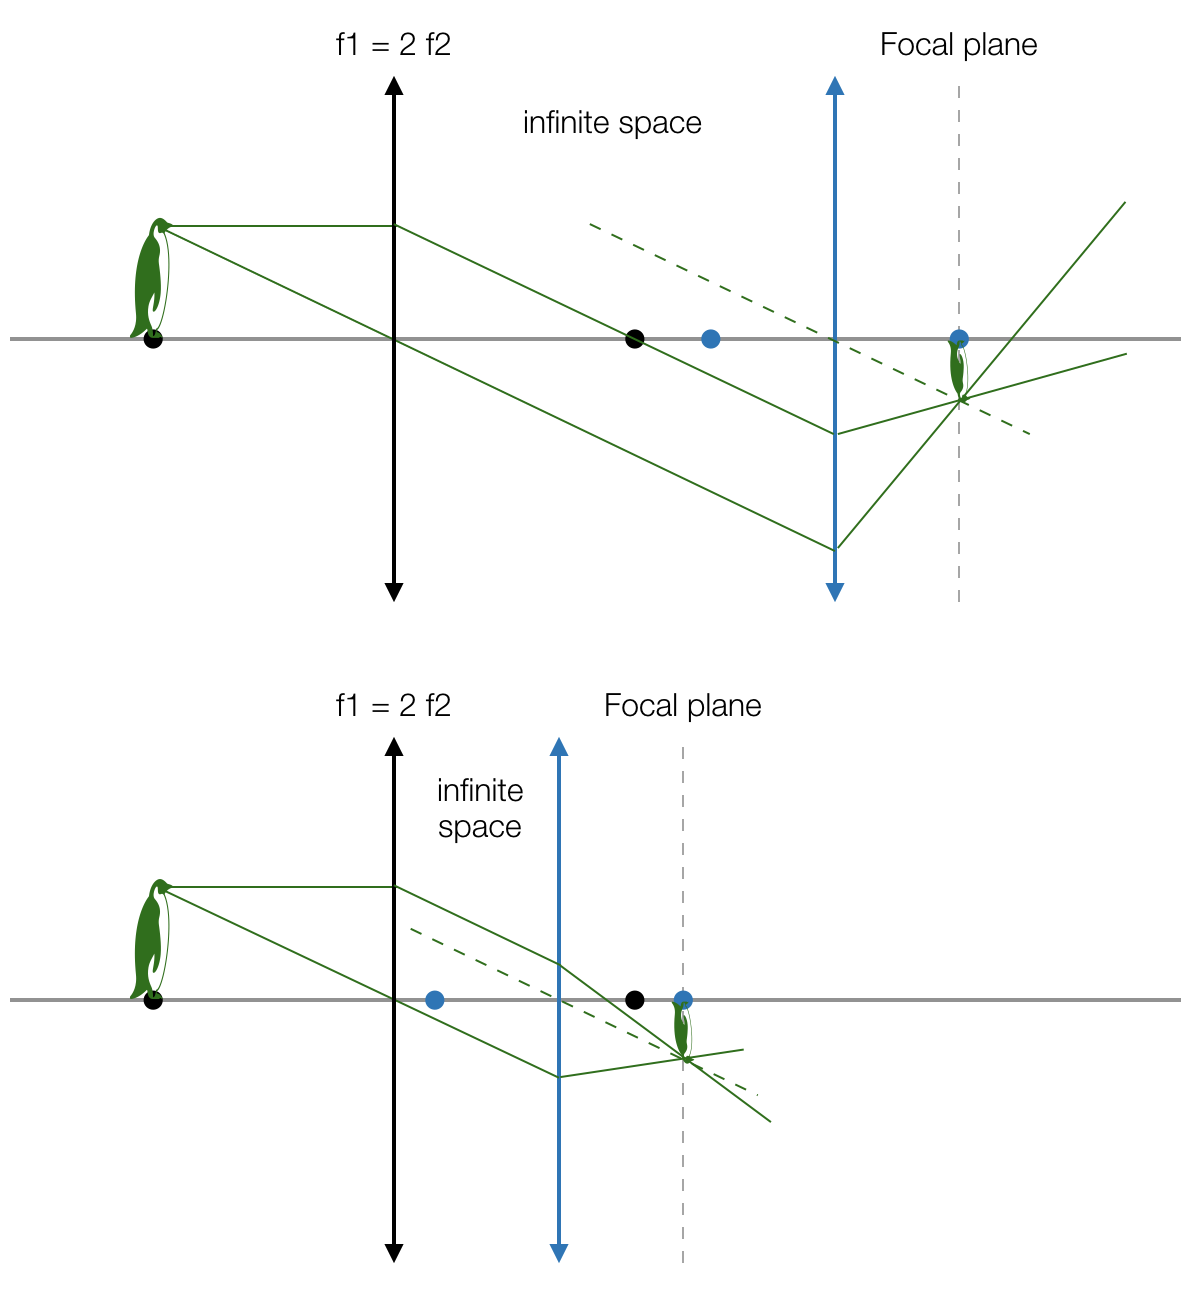
\includegraphics[width=0.7\textwidth]{figures/hint_infinite_conjugate.png}
		\caption{Illustration of the infinite space between two lenses in infinite conjugate configuration}
		\label{hint_infinite}
	\end{figure}

    
	\subsubsection{What is the use of it?}
	The two lenses form a simple microscope, where the first is the objective and the second would be called the tube lens. The infinite conjugate arrangement is useful because the image is always formed at $1f$ from the second lens, irrespective of the distance between the lenses. This means we can fix the tube lens and camera (your screen) in place. To increase magnification, we can simply switch the objective for one with a shorter focal length, and move the sample until it forms a sharp image on the camera (which means it is now at $1f$ from the objective). Moreover, it allows for filter cubes to be placed between the objective and tube lens (we will encounter those in the fluorescence practical). 

    
    \subsubsection{Building the infinite conjugate}
	We rarely rely on rulers to determine where to place optical elements. In this case, we know from our diagram that if $d_o=-f_1$, we should see an image of it at infinity. Perhaps the wall across the room is far enough? You can form an image on the wall (the image should be big now, since $m=inf$ at $d_o=-f_1$). Now you know the emitter is a bit further from the lens than $f$. Move it a tiny bit more and leave it there. 

    \clearpage
    
    %----------------------------------------------------------------------
    \subsection{Hint - Beam expanders}
    %----------------------------------------------------------------------
	\hypertarget{hintTo-expand}{}
	
	\subsubsection{Collimated light}
	Light reaching us from a star can be seen as collimated due to the extreme distance from us. The reason light emitted by an LED or light bulb cannot be collimated is because they are \emph{extended light sources} -- they are a collection of many point sources (vibrating or jumping electrons) spread out over potentially several millimeters. These individual point sources will each create a collimated beam leaving the lens at an angle. All together the resulting light beam will be expanding.

	
	\begin{figure}[h]
		\center
		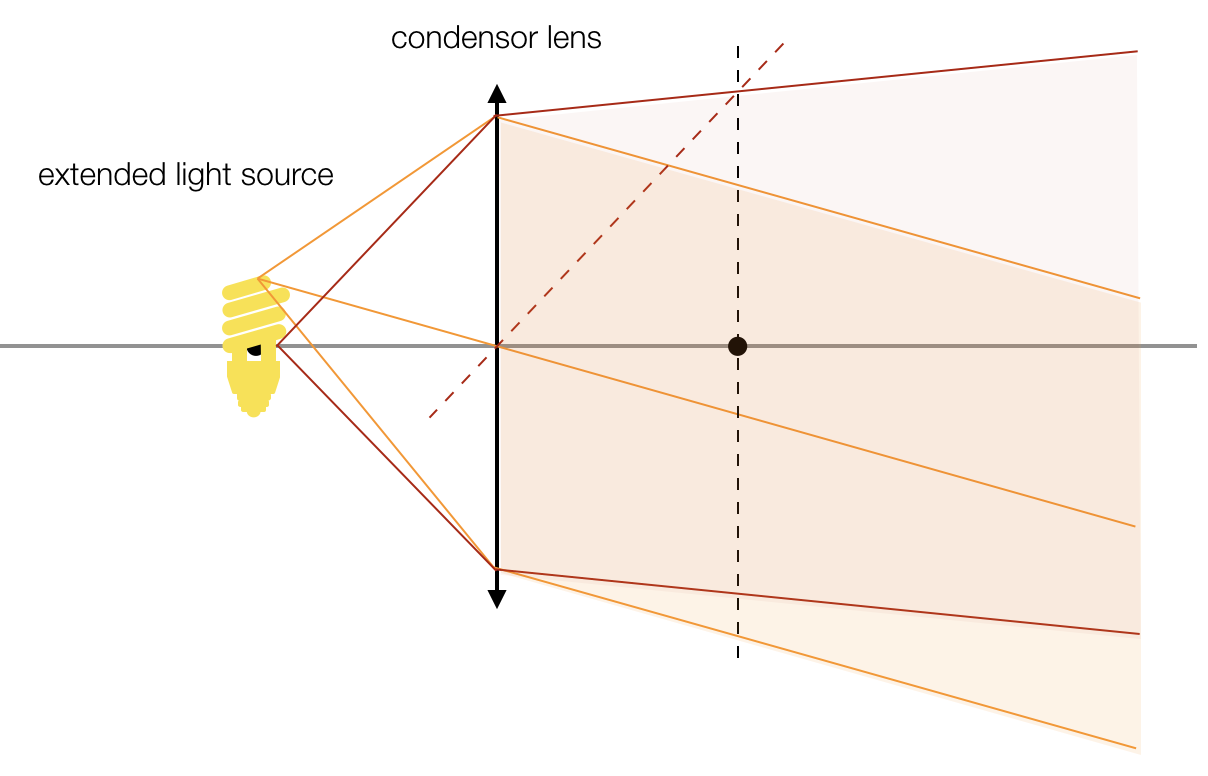
\includegraphics[width=0.65\textwidth]{figures/collimated_led.png}
		\captionsetup{width=0.65\textwidth}
		\caption{Illustration why an extended light source cannot be collimated. The yellow source is vertically offset from the focal point. The red source is too close to the lens ($d_o<f$). The dotted red ray is the helper ray needed to determine the degree of divergence.}
		\label{collimation}
	\end{figure}
	
	\subsubsection{Shrinking and expanding a beam on paper}
	Expanders can be built using either two positive lenses (Fig.~\ref{beamExpander1}) or a negative and a positive lens (Fig.~\ref{beamExpander2}). In both cases the first lens forms a point source, the light from which is collimated by the second lens. In other words, the image formed by the first lens is imaged at infinity by the second lens. You can see at a glance that the longer the focal length of the second lens, the larger the exiting beam -- if you wait twice as long, it ends up being twice as wide. 
	
	From similar triangles we get the magnification as the ratio of the two lenses:
	\begin{equation}
	\frac{d_2}{d_1}=\frac{f_2}{f_1}
	\label{eq:beamExp}
	\end{equation}
	
	\begin{figure}[h!]
		\center
		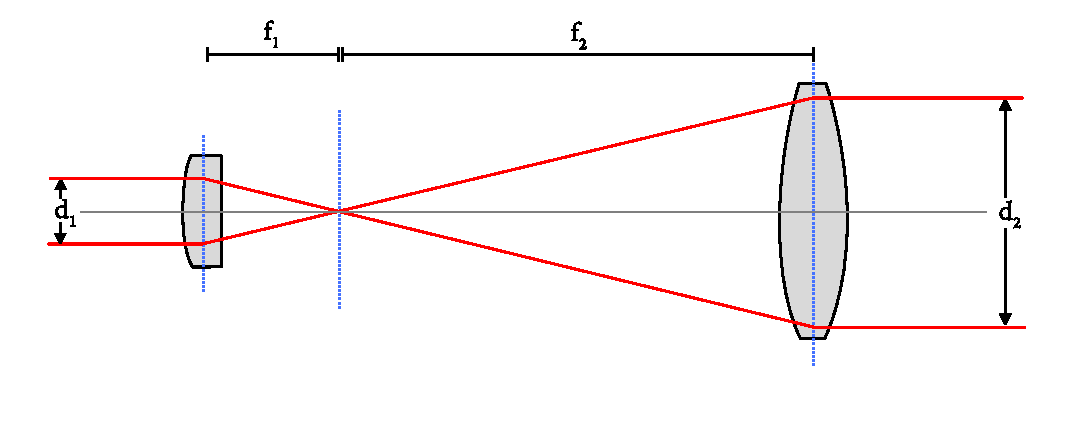
\includegraphics[width=0.6\textwidth]{beamExpander1.eps}
		\caption{Beam expander with two positive lenses.}
		\label{beamExpander1}
	\end{figure}
	
	\begin{figure}[h!]
		\center
		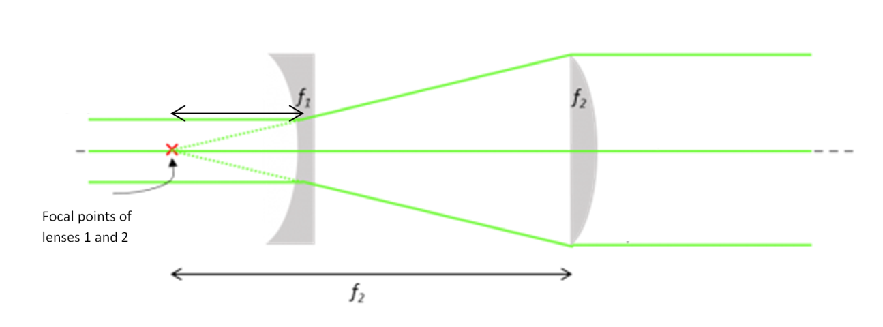
\includegraphics[width=0.6\textwidth]{beamExpander2.eps}
		\caption{Beam expander with one negative and one positive lens.}
		\label{beamExpander2}
	\end{figure}
	
	There are two advantages of the negative+positive configuration: i) it is more compact, by $2\cdot f_1$; ii) it never forms a real image of the collimated beam, that is, the light doesn't get focused to a point where small dust particles can block a large portion of it and cause the beam to `flicker'. However, that also makes the alignment more challenging, since we loose the opportunity to place an iris after lens 1 to ensure the light is on axis.

	
	\subsubsection{Building a beam expander}
	Fine alignment, as previously mentioned, is almost exclusively done `optically'. Here, we can again use the size of your room -- distance is always welcome, since it linearly amplifies any errors. Send the expanded beam across the room and make sure it stays the same size. Provided the laser pointer gives you collimated light, that means the lenses must be $f_1+f_2$ apart. Note: when measuring beam size like this, make sure the lighting conditions are similar in the two spots (just after the expander and far away on the wall) -- if there is a bit more stray light in one place, the beam will look smaller to you because of lack of contrast.

	\clearpage
	
	
	%----------------------------------------------------------------------
    \subsection{Hint - Choosing a lens}
    %----------------------------------------------------------------------
	\hypertarget{hintTo-buying}{}
	
	\subsubsection{The focusing ring}
	The job of the focusing ring is to make sure the image formed by the lens (there \emph{will} be an image unless $-f<d_o<0$) falls exactly onto the camera sensor. The only thing the ring can do to achieve this is adjusting the physical distance of the lens to the sensor. This will change where the object has to be for the sensor to be in a conjugate plane with it. On a nice lens, the acceptable range of $d_o$ is marked on the lens. Cheap lenses on cheap cameras are threaded and adjust focus by screwing closer to the chip (as opposed to a smoother internal mechanism).

	
	\subsubsection{Taking a picture to figure out $f$}
	She is onto something! Say you measure $d_o=-5m$ (remember Cartesian sign conventions). With your friend's trick, you can deduce $d_i$, since you know $m=h_i/h_o=d_i/d_o$ and the camera sensor size can be looked up. Say she is 2m tall and her image is formed onto a 20mm sensor, giving $m=-0.01$ (a minified inverted image). This means the lens sits at $d_i=50mm$ from the sensor, and using the thin lens equation we get $f=49.5mm$. 
	
	Does this surprise you? Check the blue penguin and the light blue line in Fig. \ref{fig:imageforming}: Clearly, for strong minification we need to have $d_i$ approach $1f$. Since with most camera lenses we are in that regime, it is safe to assume that the lens sits close to $1f$ from the sensor.
	
	\subsubsection{Too close to focus?}
	She can't know! We don't know the lens--sensor distance $d_i$. Here, it would need to be $d_i>52.6mm$ (we know $d_o=1m$ and $f=50mm$). In practice, manufacturers (ideally) report the closest distance at which a sharp image can be obtained as MOD or `minimum object distance'. However, your friend might have a point: given the considerations in the previous question, the sensor is probably close to $50mm$ from the lens and you will be too close to focus on your mouse.

	
	\subsubsection{Filming the pupil}
	This choice is deceptively simple. We want a detailed image of the face of the mouse. For a fixed camera position, the lenses will offer a field of view that is 5:2:1 (normalised to the $35mm$ lens, using the equation for magnification \ref{eq:mag}). The $6mm$ lens offers a larger field of view, since the fixed $d_o$ is larger with respect to its focal length (it minifies the scene more); this is why short focal length lenses are also called `wide angle lenses'. Conversely, long focal length lenses like the $35mm$ are also referred to as `zoom lenses', since they minify less and allow you to take a comparatively `close-up' shot of a distant object. Thus, at first sight, we ought to go for a long focal length lens to see the pupil clearly.
	
	
	But of course we can increase magnification by moving the camera closer to the mouse (right?), so it really depends on how much each of these lenses can adjust its focus. The default for cameras is to focus near infinity, since they are used for taking pictures of fairly distant objects ($d_o>>f$). The focus ring will then \emph{increase} $d_i$ to allow for a closer focus. Start by checking the specs of the lenses to see if the minimum object distance (MOD) is listed. If so, you can calculate the field of view size given your camera sensor size and make a decision based on that, and of course based on how far away it is practical for you to place the camera. 
	
	
	An example: the MOD listed for a $6mm$ lens is 200mm (giving $d_i<6.2mm$). The image is then 0.03 times it's actual size, so on the 5mm raspberry pi camera sensor we can fit 170mm. For the $35mm$ lens the MOD is 300mm (giving $d_i<39.6mm$), $m=0.1$ and we fit 50mm onto the chip, magnifying around 3x more. Of course, you could also go with the $6mm$ lens and `zoom in' digitally, that is, record the whole body of the mouse and crop to analyse the pupil -- just make sure you have enough pixels to see the necessary detail!
	

	Finally, imagine the setup is too small and your camera has to be placed $<$MOD from the mouse. How can you still focus on the mouse? Indeed, what you are thinking of can be purchased under the name `extension rings'. To overcome the focusing limit, these rings sit between the lens and the sensor, thereby increasing $d_i$ -- draw the ray diagram to convince yourself this solves the issue (before checking fig. \ref{fig:extension})! (Note: the lens you are using is usually `infinity corrected', meaning it is engineered to have minimal aberrations when it forms an image close to $d_i=1f$ of an object located near infinity. Increasing $d_i$ too much introduce aberrations if forming an image say at $d_i=2f$.)
	
	\begin{figure}[h]
		\center
		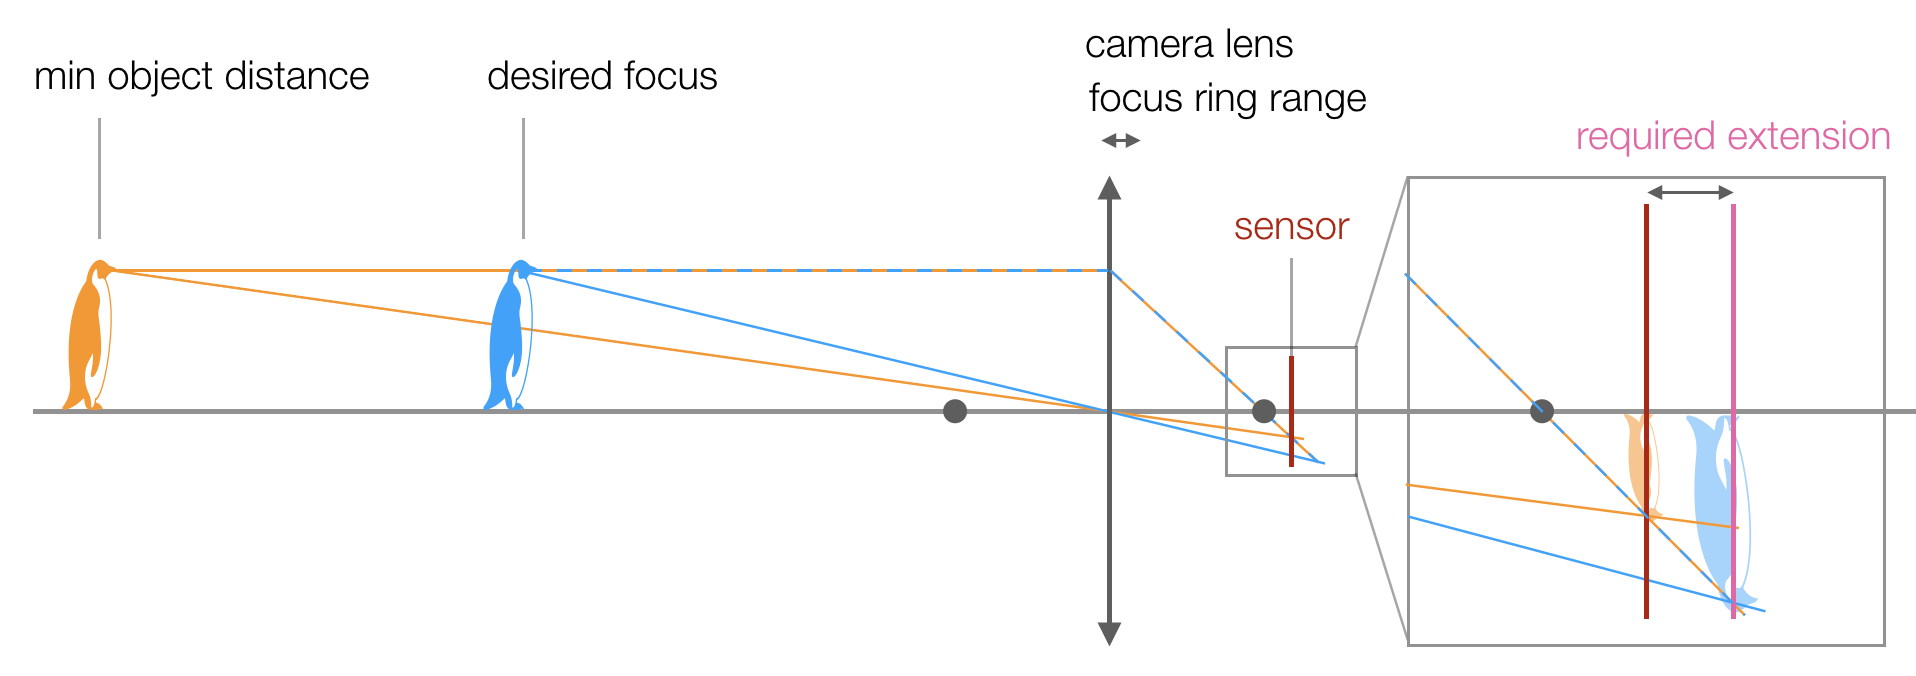
\includegraphics[width=1\textwidth]{figures/extension_ring.png}
		\captionsetup{width=1\textwidth}
		\caption{Illustration of how an extension ring works. The yellow penguin is the closest `imageable' object, but we wish to focus on the blue penguin, which form a blurry image on the sensor (light from the beak is spread out over a third of the sensor). Note how the lens is already at its most distant from the sensor, as indicated by the small arrow above it. Adding a small extension ring between the lens and the sensor allows us to shift the focal range, now including the blue penguin. Notice how the blue penguin ends up less minified -- this indicates how adding extension rings can give you a cheap `macro lens', i.e. a lens that can focus close and look at details.}
		\label{fig:extension}
	\end{figure}
	
	
	\clearpage
	
	
	%----------------------------------------------------------------------
    \subsection{Hint - A light-weight high NA lens}
    %----------------------------------------------------------------------

	


	
	%----------------------------------------------------------------------
    \subsection{Hint - A mirage for neuroscience}
    %----------------------------------------------------------------------

	
\end{document}
